\chapter{Spectroscopy on the lattice} \label{chap::Spectroscopy}

Extraction of the spectrum begins with the calculation of Euclidean two-point functions which encode the spectrum of eigenstates of lattice QCD. The functions of interest appear as matrix elements between creation and annihilation operators separated by some Euclidean distance in time. We will see that such a two-point function has a spectral representation whose time dependence is governed by the set of eigenstates of the finite volume, lattice discretized Hamiltonian, $\mathbf{H}$.  Here we present the essential details of correlator construction, a variational based analysis method which allows access to the lowest lying hadronic eigenstates, and the results from a spectroscopic calculation. 

%%%%%%%%%%%%%%%%%%%%%%%%%%%%%%%%%%%%%%%%%%%%%%%%%%%%%%%%%
%%%%%%%%%%%%%%%%%%%%%%%%%%%%%%%%%%%%%%%%%%%%%%%%%%%%%%%%%
%%%%%%%%%%%%%%%%%%%%%%%%%%%%%%%%%%%%%%%%%%%%%%%%%%%%%%%%%

\section{Correlation Functions} \label{sec::Spec:corrFunc}

Determination of the excited spectrum of QCD proceeds from the calculation of correlation functions between a \emph{basis} of creation and annihilation operators, $\{\mathcal{O}_i^\dagger\}$, separated by a distance $t$ in Euclidean time. Such a correlation function takes the form 
\begin{equation*}
C_{ij}(t) = \langle 0 | \mathcal{O}_i(t) \mathcal{O}_j^\dagger(0) | 0 \rangle 
\end{equation*}
where $|0\rangle$ denotes the vacuum. By inserting a complete set of states of the lattice discretized Hamiltonian, $\mathbf{H} | \estate{n} \rangle = E_{\estate{n}} | \estate{n} \rangle$, and time evolving the annihilation operator back to the origin, $\mathcal{O}_i(t) = e^{\mathbf{H}t} \mathcal{O}_i(0) e^{-\mathbf{H}t}$, we can decompose the correlation function into its spectral representation \footnote{In a finite volume the spectrum is discrete rather than continuous owing to the quantization of momentum ( $\mathbb{1} = \sum_{\estate{n}} \frac{1}{2E_{\estate{n}}}  | \estate{n} \rangle \langle \estate{n} |$ ). Some details of momentum conservation in a finite volume are presented in \appref{app::two-point}. } .
\begin{equation*}
C_{ij}(t) = \sum_{\estate{n}} \frac{1}{2E_{\estate{n}}} \langle 0 | \mathcal{O}_i(0) | \estate{n} \rangle \langle \estate{n} | \mathcal{O}_j^\dagger(0) | 0 \rangle e^{-E_{\estate{n}}t}
\end{equation*}

The index $\estate{n}$ runs over particle species, angular momentum, and momentum. It is worth noting that formally \emph{all} strongly interacting eigenstates, including for example the nucleus of Carbon-12, are contained in this sum. We will specialize to the case of the lowest few mesonic excitations. 

By constructing operators with good quantum numbers (e.g. total angular momentum, parity, and charge conjugation quantum numbers) we can filter the sum into excitations within a given channel. This is to say that the vacuum operator state overlaps, $ \langle \estate{n} | \mathcal{O}^\dagger(0) | 0 \rangle $, will only be non-zero if the operator $\mathcal{O}$ has the same quantum numbers as the state $\estate{n}$. 

Operators appearing in the two-point functions we consider are constructed to be gauge invariant combinations of the fundamental quark and gluon fields (gauge links).  The generic form of the operators we will use is
\begin{equation*}
\mathcal{O}_i^\dagger(t) = \sum_{\vec{x}, \vec{y} } \psibar_{\vec{x}}(t)\cdot  \mathbf{\Gamma}^i_{\vec{x} \vec{y}}(t) \cdot \psi_{\vec{y}}(t)
\end{equation*}
where $\mathbf{\Gamma}$ acts in the suppressed color and spin spaces as well as coordinate space\footnote{$\mathbf{\Gamma}$ also includes momentum projection. Later, in our three-point function analysis, we will require operators projected to be at rest as well as those projected into definite momentum.}. A two point function between two such operators may be re-expressed in terms of Wick contractions and evaluated numerically. 
\begin{align*}
 \langle 0 | \mathcal{O}_i(t) \mathcal{O}_j^\dagger(0) | 0 \rangle &= \langle 0 |\psibar_{\vec{x}}(t)\mathbf{\Gamma}^i_{\vec{x} \vec{y}}(t) \psi_{\vec{y}}(t)  \cdot \psibar_{\vec{w}}(0)\mathbf{\Gamma}^j_{\vec{w} \vec{z}}(0) \psi_{\vec{z}}(0)  | 0 \rangle \\
 &= - \trace{M^{-1}_{\vec{z}\vec{x}}(0,t)\mathbf{\Gamma}^i_{\vec{x} \vec{y}}(t)M^{-1}_{\vec{y}\vec{w}}(t,0) \mathbf{\Gamma}^j_{\vec{w} \vec{z}}(0)} \\
 & \quad\; + \trace{M^{-1}_{\vec{y}\vec{x}}(t,t) \mathbf{\Gamma}^i_{\vec{x} \vec{y}}(t)} \; \trace{M^{-1}_{\vec{z}\vec{w}}(0,0)\mathbf{\Gamma}^j_{\vec{w} \vec{z}}(0)}
\end{align*}
Here the traces are over color and spin, there are implied sums on the spatial indices. The second term involving a product of two traces is referred to as a \emph{disconnected} diagram and does not feature in the isovector correlation functions to which we specialize. 

The correlation functions are evaluated over the set of gauge configurations. We will see later in this chapter that constructing a matrix of such two point functions and inspecting the time dependence allows for robust extraction of the spectrum. The actual method we use, the variational method, becomes more powerful as one increases the redundancy of operators in a given channel of quantum numbers and, as such, we are well served by techniques that allow for both the efficient construction of a basis of operators\footnote{Details of operator construction appear in the subsequent section.} and subsequent numerical evaluation of correlation functions. Motivated by the need for a large basis in conjunction with the infrastructure to efficiently evaluate two-point functions we now turn to some of the more technical details regarding operator construction before transitioning to spectroscopic methods and results.
%Correlation functions are evaluated over the set of gauge configurations. By building up a matrix of such two point functions from we can extract spectral information via inspection of the time dependence of the matrix of correlators. Having reviewed the general mode of calculation we now turn to the details of the operator construction, smearing algorithms, and the variational calculation used in our analysis. 

%%%%%%%%%%%%%%%%%%%%%%%%%%%%%%%%%%%%%%%%%%%%%%%%%%%%%%%%%
%%%%%%%%%%%%%%%%%%%%%%%%%%%%%%%%%%%%%%%%%%%%%%%%%%%%%%%%%
%%%%%%%%%%%%%%%%%%%%%%%%%%%%%%%%%%%%%%%%%%%%%%%%%%%%%%%%%

\section{Operator Construction} \label{sec::Spec:ops}
We will only be considering the lightest few mesonic excitations and as such it is judicious to construct operators which overlap predominantly onto the low modes of the theory with reduced overlap onto higher lying excitations which are not of interest. One well-known way of improving operator overlap onto the lightest set of hadrons is `smearing' \cite{Allton:1993wc}. The thrust of these methods is to construct a new set of fields, as a combination of the fields appearing in the Lagrangian, which will be used in the operator construction. 

%\footnote{The gauge field smearing used in this analysis is non-linear while the quark field smearing is linear.}

A good smearing algorithm should be gauge covariant; we do not want to change the transformation properties of the quark fields under color gauge rotations. We would also like to preserve the properties of the quark fields under parity, charge conjugation, and rotation. The smearing function we wish to use should then preserve as many symmetries as possible while removing the presence of short range modes, which do not contribute to the long range physics we are interested in. 

Historically the method of choice is Jacobi smearing \cite{Allton:1993wc}. This method is one of several based on use of the lattice Laplacian as a smearing function. One representation   of the Laplacian is
\begin{equation*}
-\nabla^2_{\vec{x}\vec{y}}(t) = 6 \delta_{\vec{x}\vec{y}} - \sum_{j=1}^3 \left[ U_j(\vec{x},t)\delta_{\vec{x}+\hat{j},\vec{y}} + U^\dagger_j(\vec{x}-\hat{j},t)\delta_{\vec{x}-\hat{j},\vec{y}}\right]
\end{equation*}
where $U$ represents a gauge field which may be itself be constructed from a covariant gauge field smearing algorithm \footnote{Since we are working on a grid with finite spacing introduction of a derivative introduces discretization error, relative to the continuum value, which is polynomial in $a$ the lattice spacing. Various formulations of the Laplacian, based on different finite difference derivatives (e.g. forward, backward, central), will introduce different discretization effects. }. The smearing function (operator) is defined as 
\begin{equation*}
S_{\sigma,n_\sigma}(t) = \left( 1 + \frac{\sigma \nabla^2(t)}{n_\sigma}\right)^{n_\sigma} 
\end{equation*}
where the parameters $\sigma$ and $n_\sigma$ are tunable and can be used to optimize overlap onto the states of interest. It should be understood that the smearing function $S_{\sigma,n_\sigma}(t)$ has suppressed color and space indices, it is a polynomial function of the gauge covariant Laplacian, in discretized space-time the operator becomes a matrix with color and $x$-space (3-space) indices. 

When considering the effect of smearing on quark fields it is helpful  to expose the previously suppressed color and space indices of the smearing operator
\begin{equation*}
\left[S_{\sigma,n_\sigma}(t)\right]_{\vec{x}\vec{y}}^{ij} = \left[ \left( 1 + \frac{\sigma \nabla^2(t)}{n_\sigma}\right)^{n_\sigma} \right]_{\vec{x}\vec{y}}^{ij}.
\end{equation*}
The smeared quark fields are defined as 
\begin{equation*}
\tilde{\psi}_{\vec{x}}^i(t) = \sum_{\vec{y},j} \left[S_{\sigma,n_\sigma}(t)\right]_{\vec{x}\vec{y}}^{ij} \psi_{\vec{y}}^j(t)
\end{equation*}
and can be shown to be a weighted average of the quark fields amongst neighboring sites connected by parallel transporters to ensure the proper transformation under color gauge rotations.

It is helpful to consider the limit of large $n_\sigma$ (i.e. many applications of the smearing operation). In this limit the smearing function becomes $e^{\sigma \nabla^2}$ and $\sigma$ can be thought of as a smearing width. This function exponentially damps out the higher lying eigenmodes of the Laplace operator whilst retaining the lowest modes which are of interest\footnote{Recall for the $k$'th eigenvector, $\xi^{(k)}$, the Helmholtz equation is $\nabla^2\xi^{(k)} = - \lambda_k \xi^{(k)}$. Thus $e^{\sigma \nabla^2}$ damps the projection along $k$'th eigenvector with weight $e^{-\sigma \lambda_k}$. If we consider the free field case then this smearing algorithm becomes a projection onto plane waves, $\xi^{(k)} = e^{i\vec{k}\cdot \vec{x}}$ and $\lambda_k = \vec{k}^2$.  }. Indeed in the non-interacting limit the eigenfunctions of the Laplacian are plane waves, damping out the higher modes can be intuitively understood introducing a soft momentum damping on the quark fields which should not be relevant to the spectrum of low lying hadrons. 



%%%%%%%%%%%%%%%%%%%%%%%%%%%%%%%%%%%%%%%%%%%%%%%%%%%%%%%%%
%%%%%%%%%%%%%%%%%%%%%%%%%%%%%%%%%%%%%%%%%%%%%%%%%%%%%%%%%
%%%%%%%%%%%%%%%%%%%%%%%%%%%%%%%%%%%%%%%%%%%%%%%%%%%%%%%%%

\subsection{Distillation Smearing} \label{sec::Spec:ops:Distsmear}

A more modern incarnation of Laplacian based smearing, which we choose to use, is called \emph{Distillation} \cite{Peardon:2009gh}. Distillation can be thought of as a choice of quark fields to use in our operator construction. In this formulation the smearing operator is written as an outer product of some number of vectors in position and color-space. One then exploits the outer product nature of the smearing operator to factorize correlation functions into products of matrices in the distillation space. Our implementation chooses to make use of the eigenvectors of the gauge covariant Laplacian as the smearing basis. 

% It relies on the previously mention observation that as we increase the number of smearing iterations, $n_\sigma$, the resulting smearing function approaches $e^{\sigma \nabla^2}$ which damps projections against the $k$'th eigenvector as $e^{-\sigma \lambda_k}$.
 
%  The magic of distillation is the realization that instead of exponentially damping the high lying eigenmodes we can choose to simply ignore them. This is a strong statement but may be tempered by the realization that we were free all along to choose how to write down our basis of operators. 

The algorithm proceeds as follows: 
\begin{enumerate}
\item Let $V_{D}$ be the vector space of the gauge covariant three dimensional Laplacian, it is rank $N^3\times N_c$ where $N$ is the integer length of the box and $N_c = 3$,  the number of colors.  
\item Define the distillation operator, $\Box$, on timeslice $t$ as the product of an $V_D\times N_D$ matrix, $\Xi$, and its hermitian conjugate. $N_D$ is the rank of the smearing operator and is chosen to be small $N_D << V_D$. 
\begin{equation*}
\Box(t) = \Xi(t) \Xi^\dagger(t)
\end{equation*}
\item Choose the $k$'th column of $\Xi(t)$ to be the $k$'th eigenvector of $\nabla^2$, $\xi^{(k)}$, on timeslice $t$ where the eigenvectors have been ordered by eigenvalue\footnote{In principle one can choose an alternate basis of vectors as well as include some $k$ dependent function which assigns relative weights to the vectors.}. 
\begin{equation*}
\Box(t) = \Xi(t) \Xi^\dagger(t) \quad \Longrightarrow \quad \Box_{\vec{x}\vec{y}}(t) = \sum_{k=1}^N \xi_{\vec{x}}^{(k)}(t)  \xi_{\vec{y}}^{(k)^\dagger}(t) 
\end{equation*}
\item Define the distillation smeared quark fields as
\begin{equation*}
\tilde{\psi}_{\vec{x}}(t) = \sum_{\vec{y}} \Box_{\vec{x}\vec{y}}(t) \psi_{\vec{y}}(t)
\end{equation*}
\end{enumerate}

Such a smearing operator has numerous advantages, namely, the distillation operator is scalar under rotations, covariant under gauge rotations, and is parity and charge conjugation invariant.  The operator is also idempotent, $\Box^2 = \Box$, and has the property that when we increase the number of distillation operators to be the dimension of the space $V_D$ the distillation operator becomes the identity operator and the quark fields are unsmeared. 

The biggest advantage of distillation becomes evident when we consider constructing meson operators out of distillation smeared quark fields. Such an operator may be written as 
\begin{equation*}
\mathcal{O}_i(t) =  \psibar_{\vec{x}}(t)  \Box_{\vec{x}\vec{y}}(t)  \cdot  \mathbf{\Gamma}^i_{\vec{y} \vec{z}}(t)  \cdot   \Box_{\vec{z}\vec{w}}(t) \psi_{\vec{w}}(t).
\end{equation*}
Here repeated indices, as well as the suppressed color and spin indices, are summed over.  We can write a two point function composed of two such distillation smeared operators in shorthand notation (suppressing all indices) as
\begin{align*}
C_{ij}(t) = \langle 0 | \mathcal{O}_i(t) \mathcal{O}_j^\dagger(0) | 0 \rangle &= \langle 0 |\psibar_t \Box_t\mathbf{\Gamma}_t^i \Box_t \psi_t  \cdot \psibar_0 \Box_0\mathbf{\Gamma}_0^j \Box_0\psi_0  | 0 \rangle. 
\end{align*}
 After evaluating the quark field portion of the path integral the connected portion of the two point function is 
\begin{align*}
 C_{ij}(t) = -\trace{\Box_0 M^{-1}_{0t} \Box_t \Gamma^i_t \Box_t M^{-1}_{t0} \Box_0 \Gamma^j_0}.
\end{align*}
Now exposing the outer product nature of the smearing operator we see the true ingenuity of distillation smearing, namely a factorization of the correlation function into a trace over the product of a set of $N_D\times N_D$ matrices where $N_D$ is the rank of the distillation operator. Explicitly,
\begin{align*}
 C_{ij}(t) &= - \trace{\xi^{(p)}_0 \xi^{(p)\dagger}_0 M^{-1}_{0t} \xi^{(q)}_t \xi^{(q)\dagger}_t \Gamma^i_t \xi^{(r)}_t \xi^{(r)\dagger}_t  M^{-1}_{t0} \xi^{(s)}_0 \xi^{(s)\dagger}_0 \Gamma^j_0} \\
 &= -\trace{  \left[ \xi^{(p)\dagger}_0 M^{-1}_{0t} \xi^{(q)}_t  \right] \cdot \left[  \xi^{(q)\dagger}_t \Gamma^i_t \xi^{(r)}_t  \right] \cdot \left[ \xi^{(r)\dagger}_t  M^{-1}_{t0} \xi^{(s)}_0 \right] \cdot \left[ \xi^{(s)\dagger}_0 \Gamma^j_0 \xi^{(p)}_0\right] } \\
 &= - \trace{ \tau_{pq}(0,t) \cdot \Phi^i_{qr}(t) \cdot \tau_{rs}(t,0)\cdot \Phi^j_{sp}(0)},
\end{align*}
where \footnote{Here we have used the cyclic property of the trace ($\trace{ABC} = \trace{BCA}$) to ``slide'' $\xi^{(p)}_0$ around the trace.}
\begin{equation*}
\tau_{pq}(0,t) = \xi^{(p)\dagger}_0 M^{-1}_{0t} \xi^{(q)}_t \qquad \qquad \Phi^i_{qr}(t) =   \xi^{(q)\dagger}_t \Gamma^i_t \xi^{(r)}_t.
\end{equation*}

The \emph{perambulators}, $\tau_{pq}(0,t)$, describe quark propagation while the $\Phi$ encode operator construction. Of particular note is the fact that the choice of source and sink operators $\Phi$ is completely independent of the computation of the perambulators\footnote{This is not the case in traditional smearing algorithms. Older algorithms make use of `point-to-all' propagation which requires knowledge of the source or sink prior to computation of the quark propagators.}. Indeed in practice one precomputes and stores the $\tau$ and $\Phi$, this allows for the efficient calculation of a large number of correlation functions \emph{a posteriori}. A similar factorization occurs for the disconnected correlation functions, those involving the product of two or more traces, arising in isoscalar calculations. 

The essential ingredients, needed to construct our implementation of the distillation operator, are the first few eigenvectors themselves and the object $M^{-1}\xi^{(k)}$\footnote{In practice these vectors can be efficiently extracted using conjugate gradient algorithms to solve the system $Ax=b$ where $A=M$, $b=\xi^{(k)}$, and $x$ is the aptly named solution vector we desire, $M^{-1}\xi^{(k)}$.}. We again stress the value of factorization of the correlation function. In practice the rank of the distillation operator is an $\mathcal{O}(100)$ number which should be compared to the size of the full space propagator, $M^{-1}$, a matrix of rank $\mathcal{O}(10^7)$ even in modest calculations. In practice we actually only have access to $M$, computing the unsmeared correlation function would require the inversion of this entire space of this matrix. Conversely distillation only requires $\mathcal{O}(100)$ inversions. 
%%%%%%%%%%%%%%%%%%%%%%%%%%%%%%%%%%%%%%%%%%%%%%%%%%%%%%%%%
%%%%%%%%%%%%%%%%%%%%%%%%%%%%%%%%%%%%%%%%%%%%%%%%%%%%%%%%%
%%%%%%%%%%%%%%%%%%%%%%%%%%%%%%%%%%%%%%%%%%%%%%%%%%%%%%%%%

\subsection{Meson Interpolators} \label{sec::Spec:ops:MesOps}

Having reviewed the smearing algorithms and exposed the factorization of correlation functions we are now ready to turn to the construction of the operators appearing in these functions. In general the method we use for spectroscopic analysis, the variational method, makes use of a redundancy of operators within any channel of quantum numbers, the robustness of our variational solution being tied to the size and efficacy of our basis of interpolators. 

We will proceed by first considering the simplest set of operators we can construct, local fermion bilinear operators. That is, operators of generic structure $\psibar \Gamma \psi$ where $\Gamma$ is one of the sixteen Dirac matrices (e.g. $\gamma_\mu$, $\gamma_5\gamma_\mu$, $\sigma_{\mu\nu}$).  In distillation the quark fields, $\psi$, will be replaced by the smeared fields $\tilde{\psi}$, but this does not change the nature of the operator under rotations and thus the quantum numbers will be the same. We reproduce a known result, namely that the simplest local bilinears are somewhat limited in that they only allow access to $J^{PC} = 0^{-+}, 0^{++}, 1^{--}, 1^{++}, 1^{+-}$. More complicate operator constructions, considered later, will  include combinations of gauge links in addition to some Dirac structure which offer both redundancy in these channels as well as access to higher spins. 

% \footnote{On an anisotropic lattice we also have access to $0^{+-}$ due to the fact that the scalar portion of $\bar{\psi}\gamma^\delta\psi$ transforms separately from the spatial indices. (e.g. $\bar{\psi}\gamma^0\psi \sim 0^{+-}$ while $\bar{\psi}\gamma^k\psi \sim 1^{--}$} 

%%%%%%%%%%%%%%%%%%%%%%%%%%%%%%%%%%%%%%%%%%%%%%%%%%%%%%%%%
%%%%%%%%%%%%%%%%%%%%%%%%%%%%%%%%%%%%%%%%%%%%%%%%%%%%%%%%%
%%%%%%%%%%%%%%%%%%%%%%%%%%%%%%%%%%%%%%%%%%%%%%%%%%%%%%%%%

\subsubsection{Quantum Numbers of Dirac Bilinears} \label{sec::bilinearTransformations}
In the interest of conveying the essence of the derivation we make use of the familiar Minkowski space conventions in this subsection. We will show how to derive the transformation properties of Dirac bilinear operators using $\psibar \gamma^\mu \psi$ as an example. The quantum numbers $J^{PC}$, of this operator at rest are accessed by examination of its transformation under rotations ($J$), parity ($P$), and charge conjugation ($C$). We first consider the transformation of $\psibar \gamma^\mu \psi$ under rotations. 
 
A general Lorentz Transformation can be parameterized using six numbers, for example rotations using the three Euler angles and boosts along the three cartesian directions, and has the following form \cite{0201503972}.
\begin{equation*}
\Lambda = e^{-i\omega_{\mu\nu}S^{\mu\nu}}, \qquad \Lambda_{\frac{1}{2}} = e^{-\frac{i}{2}\omega_{\mu\nu}S^{\mu\nu}}, \qquad S^{\mu\nu} \equiv \frac{i}{4}\left[\gamma^{\mu},\gamma^{\nu}\right]
\end{equation*}
for $\omega_{\mu\nu}$ an anti-symmetric tensor. Under such a transformation the fermion fields become 
\begin{equation}
\psi(x) \rightarrow \Lambda_{\frac{1}{2}}\psi(\Lambda^{-1}x), \qquad \bar{\psi}(x) \rightarrow \bar{\psi}(\Lambda^{-1}x)\Lambda^{-1}_{\frac{1}{2}}
\end{equation}

Rotations are a subset of Lorentz transformations and can be parameterized\footnote{For example $\omega_{12} = -\omega_{21} = \theta$ with all other components zero is just a rotation in the $xy$-plane.} by $\omega_{\mu\nu}$ where $\omega_{0\mu} = 0$ (ie: no boosts).  We will use a general Lorentz parametrization with the understanding that the boost parameters are zero. It is sufficient to consider infinitesimal transformation to $\mathcal{O}(\omega)$ when determining the transformation laws. For small $\omega$ the operator $\psibar \gamma^\delta \psi$ transforms like 
\begin{equation*}
\psibar \gamma^\delta \psi \rightarrow \bar{\psi}\Lambda^{-1}_{\frac{1}{2}}\gamma^{\delta}\Lambda_{\frac{1}{2}}\psi = \bar{\psi}\left(1 + \frac{i}{2}\omega_{\mu\nu}S^{\mu\nu}\right)\gamma^{\delta}\left(1 - \frac{i}{2}\omega_{\rho\sigma}S^{\rho\sigma}\right)\psi + \mathcal{O}(\omega^2).
\end{equation*}
working on the term $\left(1 + \frac{i}{2}\omega_{\mu\nu}S^{\mu\nu}\right)\gamma^{\delta}\left(1 - \frac{i}{2}\omega_{\rho\sigma}S^{\rho\sigma}\right)$ we see
\begin{align*}
&\left(1 + \frac{i}{2}\omega_{\mu\nu}S^{\mu\nu}\right)\gamma^{\delta}\left(1 - \frac{i}{2}\omega_{\rho\sigma}S^{\rho\sigma}\right) \\
&\qquad\qquad= \left(\gamma^{\delta} + \frac{i}{2}\omega_{\mu\nu}\frac{i}{4}\left[\gamma^{\mu},\gamma^{\nu}\right]\gamma^{\delta}\right)\left(1 - \frac{i}{2}\omega_{\rho\sigma}S^{\rho\sigma}\right) \\
&\qquad\qquad =\left(\gamma^{\delta} + \frac{i}{2}\omega_{\mu\nu}\frac{i}{4}  \left(\gamma^{\mu}\gamma^{\nu}\gamma^{\delta} - \gamma^{\nu}\gamma^{\mu}\gamma^{\delta}  \right) \right)\left(1 - \frac{i}{2}\omega_{\rho\sigma}S^{\rho\sigma}\right).
\end{align*}
Using the formula $\gamma^{\mu}\gamma^{\nu}\gamma^{\delta} = 2\gamma^{\mu}g^{\nu\delta} - 2\gamma^{\nu}g^{\mu\delta} + \gamma^{\delta}\gamma^{\mu}\gamma^{\nu}$ we see
\begin{align*}
&\left(\gamma^{\delta} + \frac{i}{2}\omega_{\mu\nu}\frac{i}{4}  \left(\gamma^{\mu}\gamma^{\nu}\gamma^{\delta} - \gamma^{\nu}\gamma^{\mu}\gamma^{\delta}  \right) \right)\left(1 - \frac{i}{2}\omega_{\rho\sigma}S^{\rho\sigma}\right) \\
&\qquad\qquad= \left(\gamma^{\delta}\left(1 + \frac{i}{2}\omega_{\mu\nu}S^{\mu\nu}\right) - \frac{1}{2}\omega_{\mu\nu}\left(\gamma^{\mu}g^{\nu\delta} - \gamma^{\nu}g^{\mu\delta}\right)\right)\left(1 - \frac{i}{2}\omega_{\rho\sigma}S^{\rho\sigma}\right) \\
&\qquad\qquad=\gamma^{\delta} - \omega_{\mu\nu}\gamma^{\mu}g^{\nu\delta} + \mathcal{O}(\omega^2).
\end{align*}

The operator $\psibar \gamma^\delta \psi$ behaves as a Lorentz 4-vector under transformations\footnote{This is just the 4-vector encoding of the more familiar infinitesimal rotation in three dimensions, $\gamma_j \rightarrow \gamma_j  + \omega_{jk} \gamma_k$, where the matrix $\omega$ encodes the rotation parameters.} 
\begin{equation*}
\psibar \gamma^\delta \psi \rightarrow  \bar{\psi}\gamma^{\delta}\psi - \omega_{\mu}^\delta\bar{\psi}\gamma^{\mu}\psi + \mathcal{O}(\omega^2).
\end{equation*}
Equivalently, the temporal portion of this operator, $\delta=0$, transforms like a scalar while the spatial portion transforms like a vector and can be assigned to total angular momentum $J=1$. 

Under parity transformations, $\mathcal{P}$, the quark fields transform as
\begin{equation*}
\mathcal{P} \psi(t,x) \mathcal{P} = \eta \gamma^0 \psi(t,-x)\end{equation*}
where $|\eta|^2 =1$. Applying this rule to the quark fields we see the bilinear $\psibar \gamma^\delta \psi$ transforms as
\begin{equation*}
\mathcal{P} \psibar \gamma^\delta \psi \mathcal{P} = |\eta|^2\psibar \gamma^0 \gamma^\delta \gamma^0 \psi(t,-x)  = \begin{cases} 
+\psibar \gamma^\delta \psi &\mbox{for } \delta = 0 \\ 
-\psibar \gamma^\delta \psi &\mbox{for } \delta = 1,2,3. \\ 
\end{cases}
\end{equation*} 
Here we see that the operator, $\psibar \gamma^\delta \psi$, acquires the same minus sign on the spatial components as the vector $x^\mu$, thus we conclude that the bilinear transforms as a Lorentz 4-vector under parity transformations. 

The other discrete transformation we will consider, particle-antiparticle symmetry, or charge conjugation ($\mathcal{C}$) effectively changes fermions to antifermions. Under this transformation the quark and antiquark fields transform as 
\begin{equation*}
\mathcal{C} \psi \mathcal{C} = -i (\psibar \gamma^0 \gamma^2)^T \qquad \qquad \mathcal{C}\psibar\mathcal{C} = -i (\gamma^0\gamma^2\psi)^T.
\end{equation*}
Working out the charge conjugation can be a bit tricky and it is helpful to write out the spinor indices. For the vector bilinear we find 
\begin{align*}
\mathcal{C} \psibar \gamma^\delta \psi \mathcal{C} &= \mathcal{C} \psibar_\alpha \mathcal{C}\mathcal{C}\gamma^\delta_{\alpha\beta}\mathcal{C}\mathcal{C} \psi_\beta \mathcal{C} \\
& = -(\gamma^0\gamma^2\psi)^T_{\alpha} \gamma^\delta_{\alpha\beta} (\psibar \gamma^0 \gamma^2)^T_\beta \\
&= \psibar_a \gamma^0_{ab} \gamma^2_{b\beta} \gamma^\delta_{\alpha\beta}\gamma^0_{\alpha c}\gamma^2_{cd}\psi_d 
\end{align*}
Evaluating each component individually and recalling that $\gamma^0$ and $\gamma^2$ are symmetric while $\gamma^1$ and $\gamma^3$ are antisymmetric \footnote{We need to exchange $\gamma^\delta_{\alpha\beta}
$ for its transpose, $\gamma^\delta_{\beta\alpha}$.}  we find 
\begin{equation*}
\mathcal{C} \psibar \gamma^\delta \psi \mathcal{C} = \begin{cases}
\psibar \gamma^0 \gamma^2\gamma^0\gamma^0\gamma^2\psi = \psibar \gamma^0 \gamma^2\gamma^2\psi = - \psibar \gamma^0 \psi & \mbox{for } \delta = 0 \\
-\psibar \gamma^0 \gamma^2\gamma^1\gamma^0\gamma^2\psi = -\psibar \gamma^2\gamma^1\gamma^2\psi = - \psibar \gamma^1 \psi & \mbox{for } \delta = 1 \\
\psibar \gamma^0 \gamma^2\gamma^2\gamma^0\gamma^2\psi = -\psibar \gamma^0 \gamma^0\gamma^2\psi = - \psibar \gamma^2 \psi & \mbox{for } \delta = 2\\
-\psibar \gamma^0 \gamma^2\gamma^3\gamma^0\gamma^2\psi = -\psibar \gamma^2\gamma^3\gamma^2\psi = - \psibar \gamma^3 \psi & \mbox{for } \delta = 3. \\
\end{cases} 
\end{equation*}
Thus we conclude that the operator $\psibar \gamma^\delta \psi$ is has a good charge conjugation quantum number with eigenvalue $-1$ \footnote{Strictly one can only form charge conjugation eigenstates when the quark and antiquark fields are the same flavor. For two degenerate flavors charge conjugation generalizes simply to G-parity.}. For the sake of brevity we summarize the transformation properties of the sixteen fermion bilinears in \tabref{tab::JPCSimpleOps}  separating the vector and scalar positions of the 4-vectors. 

\begin{table}[hbtp]
\begin{centering}
\caption{$J^{PC}$ quantum numbers of the simplest fermion bilinears.  }\label{tab::JPCSimpleOps}
\begin{tabular}{ccccccccc}
& $\psibar \psi$ & $\psibar \gamma^5 \psi$ & $\psibar \gamma^0\psi$ & $\psibar \gamma^k\psi$ & $\psibar \gamma^5\gamma^0\psi$ & $\psibar \gamma^5 \gamma^k\psi$ & $\psibar \gamma^0 \gamma^k\psi$ & $\epsilon_{ijk} \psibar \gamma^i \gamma^j\psi$ \\ \hline
$J^{PC}$ & $0^{++}$ &$0^{-+}$ &$0^{+-}$ &$1^{--}$ &$0^{-+}$ &$1^{++}$ &$1^{--}$ &$1^{+-}$ 
\end{tabular}
\end{centering}
\end{table}

%%%%%%%%%%%%%%%%%%%%%%%%%%%%%%%%%%%%%%%%%%%%%%%%%%%%%%%%%
%%%%%%%%%%%%%%%%%%%%%%%%%%%%%%%%%%%%%%%%%%%%%%%%%%%%%%%%%
%%%%%%%%%%%%%%%%%%%%%%%%%%%%%%%%%%%%%%%%%%%%%%%%%%%%%%%%%

\subsubsection{Derivative Based Meson Operators}
As we have just seen the simple local fermion bilinear operators are limited in the sense that they restrict us to a small set of quantum numbers without very much redundancy in any given channel. In order to construct operators of higher spin and to produce multiple operators within a given symmetry channel one can consider the use of non-local operators. We consider operators of generic structure 

\begin{equation*}
\mathcal{O} \sim \psibar \Gamma \overleftrightarrow{D}_i \overleftrightarrow{D}_j \ldots \psi.
\end{equation*} 
$\overleftrightarrow{D} \equiv \overleftarrow{D} - \overrightarrow{D}$ where $D$ is a gauge covariant derivative. We have suppressed color, space, and spin indices for clarity. The use of the ``forward-backward" derivative is not strictly necessary but it simplifies the construction of operators of definite charge conjugation symmetry at non-zero momentum. Working first with continuum rotational symmetry we form a circular basis of cartesian vector-like operators and gamma matrices (e.g. $\overleftrightarrow{D}_i, \gamma_i, \epsilon_{ijk}\gamma_j\gamma_k, \ldots$),  
\begin{equation*}
\overleftrightarrow{D}_m = i\sum_k \epsilon^*_k(m) \overleftrightarrow{D}_k
\end{equation*}
for 
\begin{equation*}
\vec{\epsilon}(m) = \begin{cases} - \frac{1}{\sqrt{2}} (1,  i, 0) & \mbox{for } m = +1 \\
(0, 0 , 1) & \mbox{for } m = 0 \\
 \frac{1}{\sqrt{2}} (1, - i, 0) & \mbox{for } m = -1. \\
\end{cases}
\end{equation*}

Expressed in this basis the derivatives and vector like gamma matrices transform like $J=1$. Higher spins can be constructed by coupling components together using the standard $SO(3)$ Clebsch-Gordon symbols. For example if we couple a vector-like gamma matrix to a single derivative we can form operators of total angular momentum $J=0,1,2$ as  
\begin{equation*}
\left( \Gamma_{J=1} \times D^{[1]}_{J_D}\right)^{J,M} = \sum_{m_1,m_2} \langle 1,m_1 ; 1, m_2 | J,M\rangle \; \psibar \Gamma_{m_1} \overleftrightarrow{D}_{m_2} \psi . 
\end{equation*}
Two derivative operators may be constructed in a similar manner. We use the convention where the derivatives are first coupled together to form angular momentum $J_D = 0,1,2$, then the angular momentum from the vector-like gamma matrix is added allowing access to total angular momentum $J=0,1,2,3$. 
\begin{align*}
\left( \Gamma_{J=1} \times D^{[2]}_{J_D}\right)^{J,M}  = \sum_{\substack{m_1,m_2 \\ m_3,m_D}} & \langle 1,m_1 ; J_D, m_D | J,M\rangle \\ 
& \quad \times \langle 1,m_2 ; 1, m_3 | J_D,m_D\rangle \; \psibar \Gamma_{m_1} \overleftrightarrow{D}_{m_2} \overleftrightarrow{D}_{m_3} \psi
\end{align*}
Of particular interest in this example is the fact that the Clebsch-Gordon coefficients for $1\otimes1\rightarrow 1$ are antisymmetric in the two indices, this means the operator constructed from two gauge covariant derivatives coupled together into spin 1 is proportional to a commutator of two derivatives. In the absence of gauge fields this commutator is zero, derivatives in different directions commute. Once we promote the derivatives to the gauge covariant derivatives the commutator is proportional to the field strength tensor\footnote{$F^{\mu\nu} = \left[ D^\mu, D^\nu\right]$, since we only work with spatial derivatives we only access the spatial (magnetic) portion of the field strength tensor. } which does not vanish on non-trivial gauge configurations. 

Higher spins may be accessed in a similar manner by coupling together more derivatives. In practice we use up to three derivatives for operators projected into rest and up to two derivatives for mesons projected onto non-zero momentum. We have access to $J\leq 4$ at rest and $J\leq3$ in flight. 


%%%%%%%%%%%%%%%%%%%%%%%%%%%%%%%%%%%%%%%%%%%%%%%%%%%%%%%%%
%%%%%%%%%%%%%%%%%%%%%%%%%%%%%%%%%%%%%%%%%%%%%%%%%%%%%%%%%
%%%%%%%%%%%%%%%%%%%%%%%%%%%%%%%%%%%%%%%%%%%%%%%%%%%%%%%%%

\subsubsection{Subduction into lattice irreps} \label{Spec::Subduce}
In lattice QCD calculations the theory is discretized on a four dimensional Euclidean hyper toroid grid. This means that the full rotational symmetry of the continuum, which gives rise to angular momentum conservation and allows for the classification of eigenstates in terms of their total angular momentum $J$, is broken. Instead, we are left with the symmetry group of the cube, or equivalently the octrahedral group. At rest the single cover cubic group relevant to the integer spin mesons we consider has five irreducible representations (\emph{irreps}): $A_1,A_2,E,T_1,T_2$\footnote{The $A_1$ and $A_2$ irreps are one dimensional. The $E$ irrep has dimension two.  $T_1$ and $T_2$ are three dimensional.}. The process of distributing the various $M$ projections of a spin $J$ meson across the cubic irreps is called \emph{subduction}. The essence of the procedure reduces to taking linear combinations of the projections ($M$) to create operators which transform irreducibly under the cubic symmetry of the box
\begin{equation}
\mathcal{O}_{\Lambda,\mu} \equiv \sum_M S^{J,M}_{\Lambda,\mu}\mathcal{O}^{J,M} 
\end{equation} 
where $\Lambda$ is the cubic irrep, $A_1,A_2,E,T_1,T_2$, and $\mu$ is the ``row" of the irrep ($1\ldots \mathrm{dim}(\Lambda)$). 

 $S^{J,M}_{\Lambda,\mu}$ is a \emph{subduction matrix}, it is unitary, $\sum_{M} S^{J,M}_{\Lambda,\mu} S^{J,M*}_{\Lambda',\mu'} = \delta_{\Lambda,\Lambda'}\delta_{\mu,\mu'}$, which fixes the normalization of the subduction coefficients\footnote{The subduction coefficients for integer spin can be rephased such that all coefficients are real. This is not true in the case half integer spin.}.  The distribution of continuum spins into lattice irreps is presented in \tabref{tab::subduce} \footnote{Table reproduced from \cite{Dudek:2010wm}}. 
 
\begin{table}[htbp]
\caption{Continuum spins subduced into lattice irreps $\Lambda(\mathrm{dim})$.\label{tab::subduce}}
\begin{center}
\begin{tabular}{ccl}
$J$ & & irreps \\
\hline
$0$ & & $A_1(1)$ \\
$1$ & & $T_1(3)$ \\
$2$ & & $T_2(3) \oplus E(2)$\\
$3$ & & $T_1(3) \oplus T_2(3) \oplus A_2(1)$\\
$4$ & & $A_1(1) \oplus T_1(3) \oplus T_2(3) \oplus E(2)$
\end{tabular}  
\end{center}
\end{table}
 
 It is worth noting that, at rest, parity and charge conjugation remain good quantum numbers even in discretized space-time.
 
 A representation of the subduction matrix may be constructed in a number of different ways, here we give one possible derivation. The simplest case we can consider is a $J=0$ operator, considering \tabref{tab::subduce} this only subduces into the $A_1$ irrep. It follows that $S^{0,0}_{A_1,1} = 1$. Subduction of $J=1$ operators is also straightforward, spin 1 only subduces into the $T_1$ irrep. Here $S^{1,M}_{T_1,\mu} = \delta_{\mu,2-M}$, it is simply a relabeling of the continuum angular momentum projections. 
 
 The subduction of higher spins can be constructed with an iterative algorithm starting from the $J=0,1$ coefficients and using\footnote{Discussion and formulas reproduced from \cite{Dudek:2010wm}}
\begin{eqnarray}
\mathcal{S}^{J,M}_{\Lambda, \lambda} &=& N \sum_{\lambda_1, \lambda_2} \sum_{M_1, M_2} 
\mathcal{S}^{J_1,M_1}_{\Lambda_1, \lambda_1} \mathcal{S}^{J_2,M_2}_{\Lambda_2, \lambda_2} \nonumber \\
&& C\Bigl( \begin{array}{ccc}\Lambda & \Lambda_1 & \Lambda_2 \\ \lambda & \lambda_1 & \lambda_2\end{array} \Bigr) 
\left<J_1, M_1; J_2, M_2 | J, M \right>  ~ . \nonumber
\label{Equ:SubductionIteration}
\end{eqnarray}
Here $\langle J_1, M_1; J_2, M_2 | J, M \rangle$ is the usual $SO(3)$ Clebsch-Gordan coefficient for $J_1 \otimes J_2 \rightarrow J$ and $C\Bigl( \begin{array}{ccc}\Lambda & \Lambda_1 & \Lambda_2 \\ \lambda & \lambda_1 & \lambda_2\end{array} \Bigr)$ is the octahedral group Clebsch-Gordan coefficient for $\Lambda_1 \otimes \Lambda_2 \rightarrow \Lambda$.  $N$ is a normalization factor, fixed by the requirement that the subduction coefficients form a unitary matrix as discussed above. Explicit values of subduction coefficients, further discussion, and an alternate derivation via a group projection formula are presented in \cite{Dudek:2010wm}. 

A similar set of subduction coefficients for mesons projected onto non-zero momentum also exists\footnote{These coefficients are reproduced in \appref{app::Subduce}.}. Here the relevant symmetry group is called the \emph{little group} which are the set of rotations that leave the momentum invariant. The corresponding subduction matrices subduce the different helicity components, $\lambda$, of a spin $J$ meson into another set of lattice irreps. 
 
\begin{table}
\caption{Allowed lattice momenta on a cubic lattice in a finite cubic box, along with the corresponding little groups (the double covers relevant for integer and half-integer spin) from Ref.~\cite{Moore:2005dw,Moore:2006ng}.  We list only the single cover irreps relevant for integer spin.  Lattice momenta are given in units of $2\pi / (N a_s)$ where $n,m,p \in \mathbb{Z}^*$ are non-zero integers with $n \neq m \neq p$.  The $A$ and $B$ irreps have dimension one, $E$ two and $T$ three.  $\Dic_n$ is the dicyclic group of order $4n$. Reproduced from \cite{Thomas:2011rh}. \label{tab::littlegroups}}
\begin{center}
\begin{tabular}{c|c|l}
\textbf{Lattice} & \textbf{Little Group} & \textbf{Irreps} ($\Lambda$ or $\Lambda^P$) \\
\textbf{Momentum} & (double cover) & (for single cover) \\
\hline
$(0,0,0)$ & $\text{O}_h^D$ & $A_1^{\pm}$, $A_2^{\pm}$, $E^{\pm}$, $T_1^{\pm}$, $T_2^{\pm}$ \\
$(n,0,0)$ & $\Dic_4$ & $A_1$, $A_2$, $B_1$, $B_2$, $E_2$ \\
$(n,n,0)$ & $\Dic_2$ & $A_1$, $A_2$, $B_1$, $B_2$ \\
$(n,n,n)$ & $\Dic_3$ & $A_1$, $A_2$, $E_2$ \\
$(n,m,0)$ & $\C_4$ & $A_1$, $A_2$ \\
$(n,n,m)$ & $\C_4$ & $A_1$, $A_2$ \\
$(n,m,p)$ & $\C_2$ & $A$ \\
\hline
\end{tabular}
\end{center}
\end{table} 
 


%%%%%%%%%%%%%%%%%%%%%%%%%%%%%%%%%%%%%%%%%%%%%%%%%%%%%%%%%
%%%%%%%%%%%%%%%%%%%%%%%%%%%%%%%%%%%%%%%%%%%%%%%%%%%%%%%%%
%%%%%%%%%%%%%%%%%%%%%%%%%%%%%%%%%%%%%%%%%%%%%%%%%%%%%%%%%

\subsubsection{Cubic Symmetry}\label{Spec::Cubic}

An illustrative example of subduction is $J=2$ at rest. Here the five equivalent `rows' ($M=-2 \ldots 2$) get distributed into a three-dimensional irrep called $T_2$ and a two-dimensional irrep called $E$. Because there are only a finite number of these irreps, they must also accommodate multiple values of $J$, such that $T_2$ additionally contains parts of $J=3,4\ldots$ (see for example \tabref{tab::subduce}). 

Considering only the cubic symmetry of the lattice, and not any underlying continuum-like symmetry, we would not expect there to be any relationship between different irreps. For example a correlation function featuring operators subduced from $J=2$ into  $T_2$ takes values that need not be related to one containing $E$ operators. The correlation functions we extract feature  eigenstates of the finite volume Hamiltonian, the different quantum numbers correspond to different \emph{irreducible} representations, there is no symmetry which links them.

However, were there really to be no relation, we could hardly claim to be approximating QCD in a realistic manner. In practical calculations it should be the case that through a combination of sufficiently fine lattice spacing, reduction of discretization artifacts through improvement of the action \cite{Symanzik:1983dc}, and interpolation of hadrons using operators smoothed over many lattice sites \cite{Davoudi:2012ya}, that the continuum symmetry is manifested to a good approximation with only small deviations. 

For example we might expect to see a relation between $T_2$ and $E$ correlation functions corresponding to them originating from the same $J=2$ meson. In previous two-point function calculations we have observed that the rotational symmetry of the continuum theory is clearly visible in relations amongst the irreps both for eigenstate masses and the values of matrix elements $\big\langle 0 \big| \mathcal{O}_{\Lambda \mu}^{[J]} \big| \mathfrak{n} \big\rangle$ \cite{Dudek:2009qf, Dudek:2010wm}.  

Observation of this approximate restoration of rotational symmetry, present in the continuum theory, indicates that the different eigenstates residing in the $E$ and $T_2$ irreps may be faithfully assigned to different angular momentum projections of a spin $J=2$ meson\footnote{For states lying above two-particle kinematic thresholds the boundary can have an effect and the situation becomes more complicated. A set of methods, generically referred to as L{\"u}scher methods, see for example references \cite{Kim:2005gf,Luscher:1986pf,Rummukainen:1995vs} ,allow one to extract information about two-particle infinite volume scattering below three particle threshold from lattice two-point correlation functions. These methods are beyond the scope of this manuscript. We do not address them further.}. We will make use of this feature when it comes time to explore three-point functions later in this dissertation. 


%%%%%%%%%%%%%%%%%%%%%%%%%%%%%%%%%%%%%%%%%%%%%%%%%%%%%%%%%
%%%%%%%%%%%%%%%%%%%%%%%%%%%%%%%%%%%%%%%%%%%%%%%%%%%%%%%%%
%%%%%%%%%%%%%%%%%%%%%%%%%%%%%%%%%%%%%%%%%%%%%%%%%%%%%%%%%

\section{Correlator Construction and Analysis} \label{sec::Spec:corrConstruct}
We extract the spectrum via the calculation of a set of correlation functions between the distillation smeared creation and annihilation operators previously described. The correlation functions take the generic form 
\begin{equation*}
C_{ij}(t) = \langle 0 | \mathcal{O}_i(t) \mathcal{O}_j^\dagger(0) | 0 \rangle, 
\end{equation*}
where $|0\rangle$ denotes the vacuum. As described earlier we time evolve the annihilation back to the origin and insert a complete set of states yielding a spectral decomposition of the correlation function\footnote{This form of the spectral representation is valid provided $t << L_t$ where $L_t$ is the temporal length of the box. },
\begin{equation}
C_{ij}(t) = \sum_{\estate{n}} \frac{1}{2E_{\estate{n}}} \langle 0 | \mathcal{O}_i(0) | \estate{n} \rangle \langle \estate{n} | \mathcal{O}_j^\dagger(0) | 0 \rangle e^{-E_{\estate{n}}t} \label{eqn::spec_rep_1}.
\end{equation}
We remind the reader that the discrete nature of the identity operator follows from performing the calculation in a finite volume. 

The \emph{variational method} for spectral extraction, which we use throughout, takes advantage of the redundancy of operators within the basis we described previously. The crux of the method reduces to the intuitive notion that there should be a particular linear combination of operators within our basis that is most suited to interpolate the lightest state of the spectrum, another linear combination that optimally interpolates the first excited state, a third combination for the second excited state and so on. 

The method is akin to the Rayleigh-Ritz method in ordinary Quantum Mechanics were one attempts to diagonalize the Hamiltonian in a basis of well motivated trial wave functions when an analytic solution is overly complicated. Here we attempt to diagonalize the exponentiation of the Hamiltonian in a trial basis of well motivated operators that we believe resemble the low lying eigenstates of the theory. 

Mathematically the method arises from a variational optimization problem within a set of trial weights -- we want to maximize the signal to produce, for example, a pion within a basis of operators. More practically, it requires us to solving a generalized eigenvalue problem of the form 
\begin{equation}
C(t)v^{(\estate{n})}(t) = \lambda_{\estate{n}}(t) C(t_0) v^{(\estate{n})}(t). \label{eqn::GEVP}
\end{equation}

$\lambda_{\estate{n}}(t)$ is called a \emph{generalized eigenvalue}, $\lambda_{\estate{n}}(t_0) = 1$. The \emph{generalized eigenvectors}, $v^{(\estate{n})}$, are orthogonal on a metric, $v^{(\estate{n})\dagger} C(t_0) v^{(\estate{m})} = \delta_{\estate{n},\estate{m}}$. For large times the generalized eigenvalues behave like $\lambda_{\estate{n}}(t) \sim e^{-E_{\estate{n}}(t-t_0)}$ \cite{Blossier:2009kd,Luscher:1990ck}. 

We present a derivation of the variational method, cast as a solution to an optimization problem, in \appref{app::GEVP} where we show that this method produces the best, in a variational sense, linear combination of operators to interpolate a single eigenstate of the finite volume Hamiltonian. 

The spectral representation of the correlation function, \eqnref{eqn::spec_rep_1}, can be rewritten in terms of  \emph{operator overlaps}, $Z_i^{\estate{n}} \equiv \langle \estate{n} | \mathcal{O}^\dagger_i | 0 \rangle$, where we have chosen the phases on the operators such that all overlaps are real numbers\footnote{This is a choice, generically the definition of operators appearing in Euclidean correlation functions may be rephased such that all two-point correlation functions are real. The more general form of the spectral representation is $C_{ij}(t) = \sum_{\estate{n}} \frac{Z_i^{\estate{n}*}Z_j^{\estate{n}}}{2E_{\estate{n}}} e^{-E_{\estate{n}}t}$.}, as 
\begin{equation}
C_{ij}(t) = \sum_{\estate{n}} \frac{Z_i^{\estate{n}}Z_j^{\estate{n}}}{2E_{\estate{n}}} e^{-E_{\estate{n}}t} \label{eqn::spec_rep_2}.
\end{equation}
These operator overlaps are time independent numbers which measure the strength with which an operator creates an eigenstate of the Hamiltonian and are related to the generalized eigenvectors via $Z_i^{\estate{n}} = \sqrt{2E_{\estate{n}}} e^{E_{\estate{n}}t_0/2} v^{(\estate{n})}_j C_{ji}(t_0)$
% \footnote{In practice the \emph{extracted} $Z_i^{\estate{n}}$ actually contain some residual time dependence, arising from excited state contamination, which may be fit away.}.

The orthogonality condition on the generalized eigenvectors, $v^{(\estate{n})\dagger} C(t_0) v^{(\estate{m})} = \delta_{\estate{n},\estate{m}}$, also proves to be very powerful in the extraction of near degenerate states, the resolution of which would be complicated by only considering their time dependence. Simply put there are different linear combinations of operators for degenerate states, the different linear combinations orthogonal on the metric $C(t_0)$.  Use of the variational method in conjunction with an extensive basis capable of supporting the spectrum of states allows us to resolve near degeneracies.

Naive inspection of the orthogonality condition also suggests a range of validity of the variational solution. The generalized eigenvectors are forced, by the method, to be orthogonal on the metric $C(t_0)$ -- this is an approximation to the `true orthogonality', which is defined between a much much larger number of states and operators. One then realizes that $t_0$ should be chosen to be large enough that the correlation functions are dominated by the lightest $\mathrm{dim}(C)$ states, the higher excitations having decayed away exponentially, the signals being in a loose sense numerically small enough to neglect\footnote{In actual calculation we explore a number of $t_0$ values and observe that after a sufficiently long time the spectrum tends to `settle', the solution then remaining stable until statistical noise becomes troublesome enough to spoil the data.}. 

The orthogonality condition then implies one should simply push $t_0$ out to larger and larger values in order to further damp out states with energies larger than $E_{\estate{n}'=\mathrm{dim}(C)}$. In practice this approach tends to be unreasonable. We work on a finite set of gauge configurations and so each estimate in time of the correlation function also has some variance associated with it. A general rule of thumb in lattice calculations is that the signal to noise ratio becomes smaller as one considers correlators across longer and longer times\footnote{The signal to noise on correlators typically decreases for all correlators except those featuring the ground state, the pion.}.  As we can see from \eqnref{eqn::GEVP} this noise will also enter into the variational solution and thus the orthogonality condition, we do not want to make $t_0$ so large that the statistical noise spoils the orthogonality and thus the solution. 

%%%%%%%%%%%%%%%%%%%%%%%%%%%%%%%%%%%%%%%%%%%%%%%%%%%%%%%%%
%%%%%%%%%%%%%%%%%%%%%%%%%%%%%%%%%%%%%%%%%%%%%%%%%%%%%%%%%
%%%%%%%%%%%%%%%%%%%%%%%%%%%%%%%%%%%%%%%%%%%%%%%%%%%%%%%%%
%\subsection{$\chi^2$ reconstruction} \label{sec::Spec:corrConstructPcorr} -- kill this, too much to digest
%
%The choice of $t_0$ is something of a dark-art, we work in an economy in which we trade statistical precision for false orthogonality. In order to provide a mathematical justification of our choice of $t_0$ we define a chi-square-like quantity which allows us to gauge how well an variational solution describes our two-point correlation functions. For any choice of $t_0$ we solve the generalized eigenvalue problem which produces as set of energies (via fits to the principal correlators described later) and operator overlap values. With these in hand we can reconstruct any element of the correlation matrix using \eqnref{eqn::spec_rep_2}. The chi-square-like quantity is defined as 
%\begin{align}
%\label{eqn:chisq}
%\chi^2 &= \frac{1}{\frac{1}{2}N\left(N+1\right)\left(t_{max}-t_0\right) -\frac{1}{2}N\left(N+3\right)} \notag\\
%&\quad\times\sum_{i,j\ge i}\sum_{t,t^{\prime}=t_0+1}^{t_{max}}\left(C_{ij}(t) - C_{ij}^{\mathrm{recon.}}(t)\right)\mathbb{C}_{ij}^{-1}(t,t^{\prime}) \left(C_{ij}(t^{\prime}) - C_{ij}^{\mathrm{recon.}}(t^{\prime})\right).
%\end{align}
%Where $N = \mathrm{dim}(C)$ and $\mathbb{C}$ is the timeslice covariance matrix for the correlator element $C_{ij}$. An optimal value of $t_0$ can be obtained by minimizing this chi-square-like quantity.  In practice we choose to solve the generalized eigenvalue problem for multiple values of both $t$ and $t_0$. For each $t_0$ an optimal $t_Z$, $t_Z > t_0$, is chosen, via the chi-square-like quantity. The chi-square values from multiple $t_0$'s are then compared in order to extract the variational best solution.  
%
%Deferring the details of extraction of the spectrum and overlaps to the next two sections we now present a brief overview of the actual $\chi^2$ fitting and reconstruction procedure just outlined using the $T_1^{--}$ irrep which contains $J^{PC}=(1,3,4,\ldots)^{--}$ mesons, we specialize to the $I=1$ case. 
 %
% \begin{figure}[htbp]
%\begin{centering}
%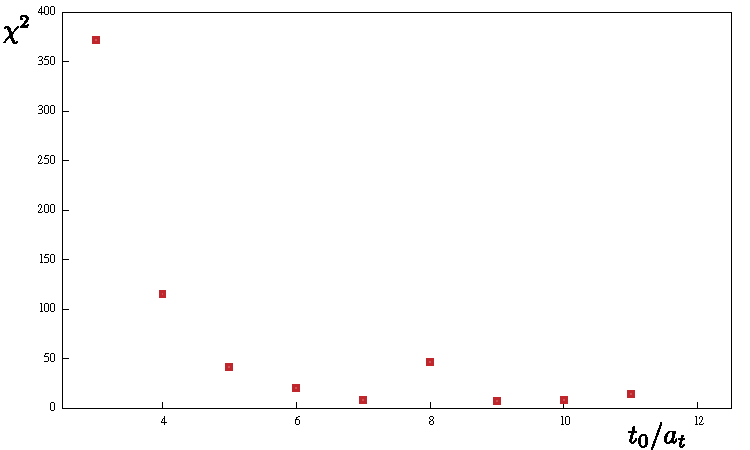
\includegraphics[width=0.8\linewidth]{figures/ChisquareT1mP/chisquare.pdf}
%\caption{ A $\chi^2$-like quantity in the $\Lambda^{PC} = T_1^{--}$ irrep for isovector correlators. \label{fig::ChisqT1mP} {\color{red} update to $A_1^{-+}$}}. 
%\end{centering}
%\end{figure}
%
%
%{\color{blue} RECONSTRUCTION PLOTS AND MORE WORDS}

 
 
%%%%%%%%%%%%%%%%%%%%%%%%%%%%%%%%%%%%%%%%%%%%%%%%%%%%%%%%%
%%%%%%%%%%%%%%%%%%%%%%%%%%%%%%%%%%%%%%%%%%%%%%%%%%%%%%%%%
%%%%%%%%%%%%%%%%%%%%%%%%%%%%%%%%%%%%%%%%%%%%%%%%%%%%%%%%%


\subsection{Principal Correlators} \label{sec::Spec:corrConstructPcorr}
The actual details of the implementation of our variational solution in terms of Singular Value Decomposition is discussed along with the derivation in \appref{app::GEVP}. We now turn to the details of spectral extraction from the \emph{principal correlators}, $\lambda_{\estate{n}}(t)$. The principal correlators can be shown by perturbation theory \cite{Blossier:2009kd} to behave asymptotically like
\begin{equation*}
\lambda_{\estate{n}}(t) \sim e^{-E_\mathfrak{n}(t-t_0)} + \mathcal{O}(e^{-E_{\estate{N+1}}t}).
\end{equation*}
Here, for a basis of $N$ operators, $E_{\estate{N+1}}$, is the energy of the $N+1$'th state.  The corrections, as expected, are proportional to the exponentiation of the energies of states that lie outside the reach of our variational basis, the smallest of which produces the largest correction. 

In practice we fit the principal correlators to the form 
\begin{equation*}
\lambda_{\estate{n}}(t) = (1-A_{\estate{n}})e^{-E_\estate{n}(t-t_0)} + A_{\estate{n}}e^{-E'_\estate{n}(t-t_0)}
\end{equation*}
where the fit parameters are $A_{\estate{n}}$, $E_{\estate{n}}$, and $E'_{\estate{n}}$. The second exponential term is present to help stabilize the fit and allows us to consider the behavior of the principal correlator at smaller times. We require the energy of the second exponential, $E'_\estate{n}$ to be larger than  $E_\estate{n}$ typically finding in practice that $E'_\estate{n}$ is of roughly the same size as $E_\estate{N}$ (i.e. it is of the size of the energy of states lying just outside the reach of our basis of operators). 

We plot a subset of principal correlators, extracted in this analysis, along with their fits, in the left and right panels of  \figref{fig::PcorrLevel}. The dominant time dependence, due to state $\estate{n}$, has been divided out such that the correlator becomes flat at the point the fit becomes dominated by the single state of interest. Empirically the importance of the second exponential becomes smaller as one increases the value of $t_0$. Further, in agreement with the perturbative analysis, the mass scale of the second exponential becomes larger than $E_\estate{N}$, $\estate{N} = \mathrm{dim}(C)$. At too early values of $t_0$ this is not necessarily true, and indication that we are forcing an incorrect orthogonality relation as discussed previously. 

\afterpage{
 \begin{figure}[htbp]
\begin{centering}
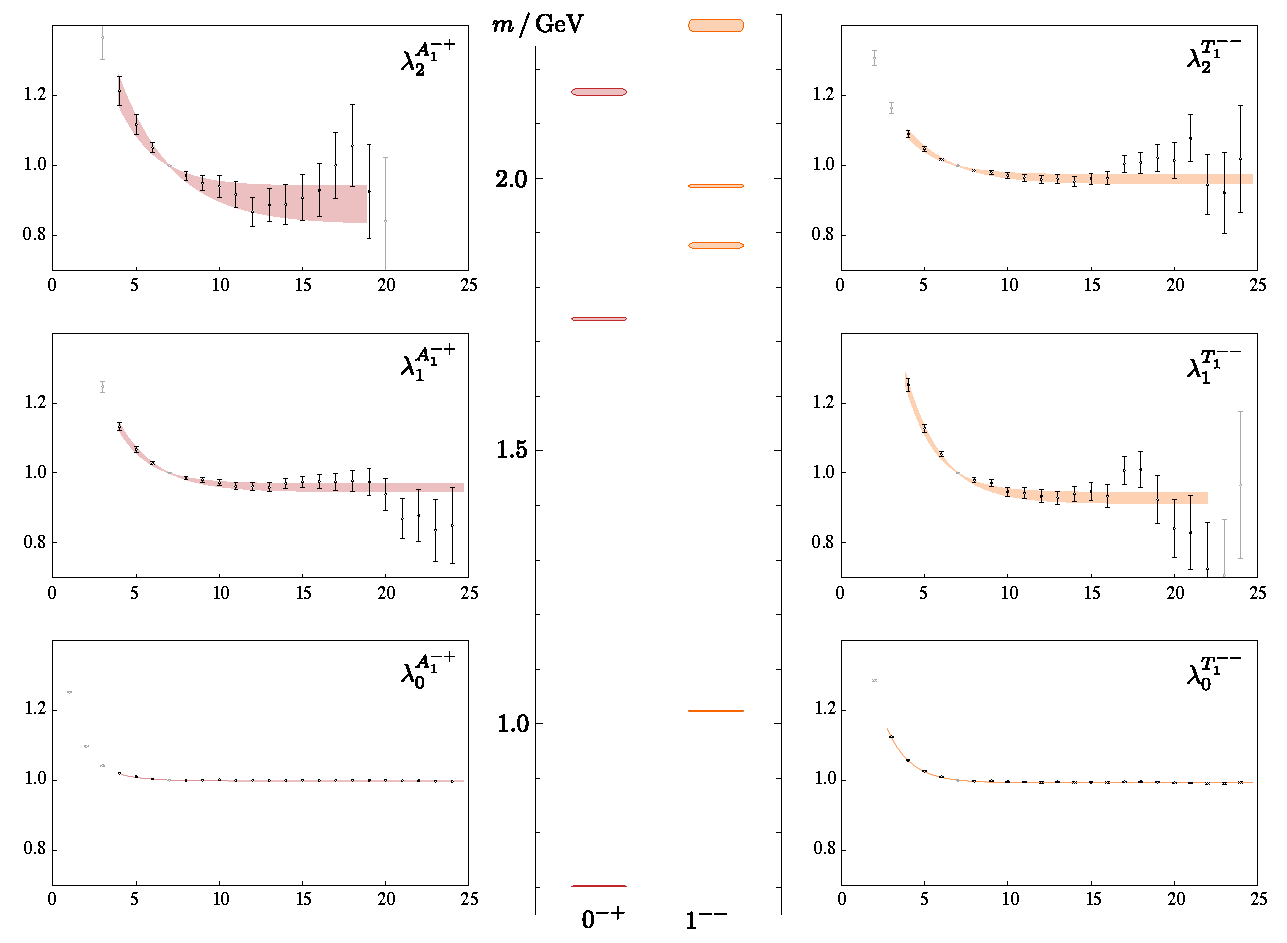
\includegraphics[width=\linewidth]{figures/PrinCorrT1mPA1mM/LevelDiagramWithT1mP_A1mM_PCorrs.pdf}
\caption{ Principal Correlators in the  $\Lambda^{PC} = A_1^{-+}$ and $T_1^{--}$ irreps containing $J^{PC}= 0^{-+}$ and $1^{--}$ mesons. We plot $e^{E_{\mathfrak{n}}(t-t_0)}\lambda_{\mathfrak{n}}(t)$. \label{fig::PcorrLevel}}
\end{centering}
\end{figure}
\clearpage
}



%%%%%%%%%%%%%%%%%%%%%%%%%%%%%%%%%%%%%%%%%%%%%%%%%%%%%%%%%
%%%%%%%%%%%%%%%%%%%%%%%%%%%%%%%%%%%%%%%%%%%%%%%%%%%%%%%%%
%%%%%%%%%%%%%%%%%%%%%%%%%%%%%%%%%%%%%%%%%%%%%%%%%%%%%%%%%


\subsection{Continuum Symmetries} \label{sec::Spec:corrConstructContSym}
As discussed previously, it should be possible through appropriate smearing, construction of operators with good continuum symmetry, and a reduction of discretization effects via improvements to the action and a sufficiently fine mesh, to restore continuum rotational symmetry to a good approximation with only small deviations. We do in fact see this apparent restoration in our lattice calculations. In \figref{fig::RotSymT1mP} we plot a correlation matrix for $\Lambda^{PC} = T_1^{--}$, organized by the continuum spin-$J$ of each operator, and normalized such that the diagonal elements are unity. We see, in explicit calculation, a nearly block diagonal matrix, an indication that the underlying continuum symmetry is approximately restored. 

\afterpage{
 \begin{figure}[htbp]
\begin{centering}
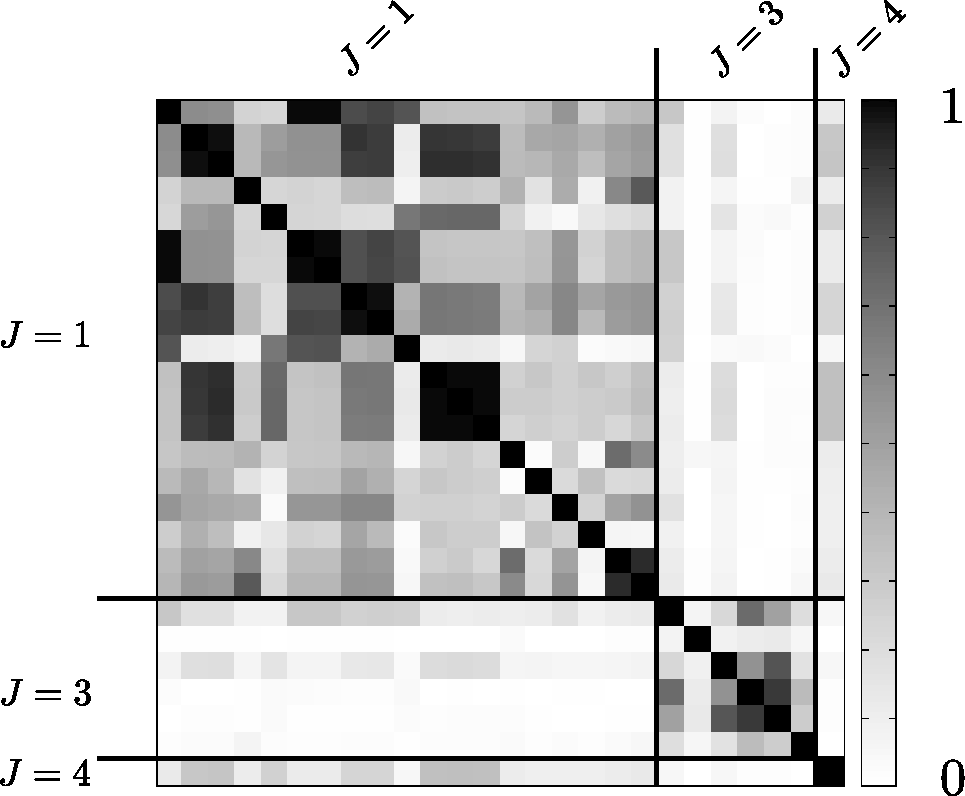
\includegraphics[width=0.8\linewidth]{figures//EmergentRotationalSymmetryT1mP/MatrixPlotLabelsCrop.pdf}
\caption{ Approximate restoration of rotational symmetry in the $\Lambda^{PC} = T_1^{--}$ irrep. We plot the normalized correlation matrix, $|C_{ij}/\sqrt{C_{ii}C_{jj}}|$ on timeslice 5. Operators subduced from spin 1 appear first followed by those subduced from spin 3 and then spin 4. \label{fig::RotSymT1mP}}
\end{centering}
\end{figure}
\clearpage
}

%%%%%%%%%%%%%%%%%%%%%%%%%%%%%%%%%%%%%%%%%%%%%%%%%%%%%%%%%
%%%%%%%%%%%%%%%%%%%%%%%%%%%%%%%%%%%%%%%%%%%%%%%%%%%%%%%%%
%%%%%%%%%%%%%%%%%%%%%%%%%%%%%%%%%%%%%%%%%%%%%%%%%%%%%%%%%


\subsection{State Identification} \label{sec::Spec:corrConstructStateIdent}

\afterpage{
 \begin{figure}[htbp]
\begin{centering}
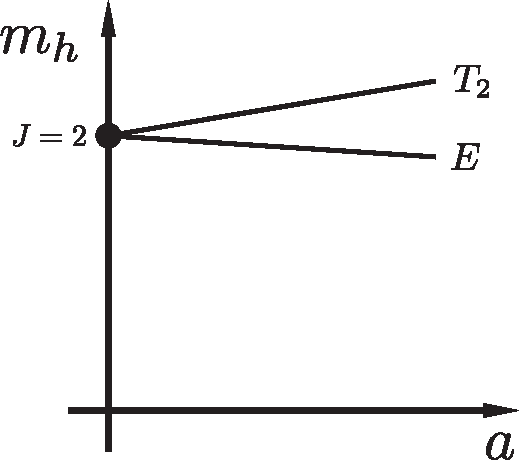
\includegraphics[width=0.3\linewidth]{figures/ContinuumExtrapolationMass/ContinuumExtrapolation.pdf}
\caption{A toy continuum limit on a $J=2$ meson. In general the extrapolation to the continuum limit may also include higher powers of the lattice spacing $a$.  \label{fig::contExtrapMass}}
\end{centering}
\end{figure}
\clearpage
}

Having identified an approximate restoration of rotational symmetry we can ask the question ``Can we identify the continuum $J^{PC}$ quantum numbers of a state from our lattice calculation?" Formally the most rigorous method to determine the spin of a state would be to perform a set of lattice calculations on successively finer meshes and then extrapolate the result to the continuum limit in which the discretization is removed. Such an extrapolation would involve a fit of the lattice masses to a function that is polynomial in $a$, the lattice spacing. One expects that after performing such a fit patterns of degeneracies would emerge, according to the patterns of subduction, and the result would be free of the discretization effects present in any single calculation. For example a spin-2 meson would appear as a degenerate set of energies in the $T_2$ and $E$ irreps (as in \figref{fig::contExtrapMass}), a spin-3 state as a degeneracy across $T_1$, $T_2$, and $A_2$, and so on. Such extrapolations have indeed been performed in pure gauge theory, $SU(3)$ Yang-Mills Theory, in the extraction of the low-lying glueball spectrum  \cite{Morningstar:1999rf}. 

\afterpage{
\begin{figure}[htbp]
\begin{centering}
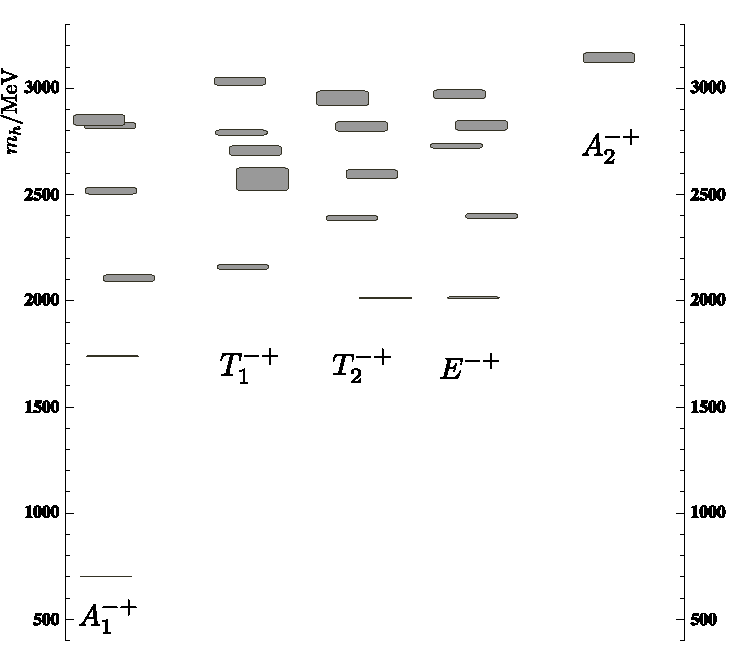
\includegraphics[width=0.8\linewidth]{figures/LatticeSpectrum743/BoxPlotUnlabeledmM.pdf}
\caption{ $\Lambda^{PC} = (A_1,T_1,T_2,E,A_2)^{-+}$ $SU(3)_F$ spectrum. \label{fig::LatticemMSpec743Raw}}
\end{centering}
\end{figure}
\clearpage
}

This procedure, applied to hadrons, is more complicated. Firstly it relies on a series of calculations on finer and finer meshes and thus comes at a large computational cost. Additionally one must simulate at a fixed quark mass, a quantity which has non-trivial dependence on the lattice spacing, thus one has complications associated with generating the required lattices beyond just the price tag. Even more troublesome however is the degree of near degeneracy manifest in the continuum spectrum when organized in terms of $J^{PC}$. When we move to the lattice the problem of degeneracy is vastly magnified, we exchange an infinite number of irreducible representations, spin-J, for the finite number of irreps of the cube. This means that the extracted spectrum becomes significantly more dense and would require statistical precision beyond that which we show here\footnote{The prototypical example of the difficulty in level identification comes from considering the subduction patterns of a $J^{PC} = 4^{++}$ meson. The fingerprint of such a continuum state would be nearly degenerate energy levels lying in $(A_1,T_1,T_2,E)^{++}$. This fingerprint is not however unique. $J^{PC} = (0,1,2)^{++}$, corresponding to a $^3P_J$ multiplet would have the same pattern. Further, on the basis of the quark model outlined earlier, we would also expect these states to also be nearly degenerate.} .  

In order to demonstrate the density of states in any given irrep we plot the spectrum of states obtained by considering $\Lambda^{PC} = (A_1,T_1,T_2,E,A_2)^{-+}$ mesons in \figref{fig::LatticemMSpec743Raw}. While the ground states in any given channel are readily identified we see the spectrum becomes fairly dense once one considers excited states. The calculation we present is performed at the $SU(3)_F$ point where all of the quarks are tuned approximately to the strange quark mass. 

%Further, this calculation is being performed at the $SU(3)_F$ point where all of the quarks are tuned approximately to the strange quark mass. %As one moves toward the physical point the constituent $u$ and $d$ quarks become lighter, multi-particle states become important, and the spacing between levels begins to shrink. 

To alleviate the difficulties with spin identification it would be useful to have a procedure which is effective at only a single spacing. This spacing should be fine enough that the spectrum exhibits, to a sufficient degree, the underlying rotational symmetry present in QCD. As shown in \figref{fig::RotSymT1mP} the lattices we employ, coupled with appropriate smearing and operator construction, appear to manifest the requisite underlying symmetry. 

The procedure, first demonstrated in \cite{Dudek:2009qf}, which we employ, makes use of both the spectrum and the operator state overlaps,  $Z_i^{\estate{n}} \equiv \langle \estate{n} | \mathcal{O}^\dagger_i | 0 \rangle$, to identify the continuum $J^{PC}$ quantum numbers. As mentioned previously, our operator basis is constructed to fully respect cubic symmetry. However, from \figref{fig::RotSymT1mP}, it is also apparent that these operators contain a `memory' of the continuum spin from which they were subduced\footnote{If they did not there would be no block diagonal sub structure in  \figref{fig::RotSymT1mP}.}.  The correlation matrix appears to be approximately block diagonal when the operators are ordered according to the spin from which they were subduced. %\footnote{In the case of $J=4$, featuring three derivatives, the symmetry is not as good. Two and three derivative operators are dimension 5 and 6 respectively, under renormalization these higher mass dimension operators can mix with lower mass dimension operators generating effects that scale like the inverse of the lattice spacing. These renormalization artifacts, while present, are not so large as to spoil the method. We expect that the use of smeared fields suppressed these dimensional mixings as they are most sensitive to the high energy physics that smearing removes. The lattice only serves to regulate the quantum field theory; renormalization must be dealt with separately.}. 

Motivated by the block diagonal nature of the correlation matrix we propose to use the operator overlaps, $Z_i^{\estate{n}} \equiv \langle \estate{n} | \mathcal{O}^\dagger_i | 0 \rangle$, in order to assign, to each state in our spectrum, an integer continuum spin, $J$. 

The essence of the method relies on the observation that operator overlaps should be degenerate in each irrep up to discretization artifacts. Our operators are constructed to be of definite spin, $\langle 0 | \mathcal{O}^{J,M} | J',M' \rangle = Z^{[J]}\delta_{J,J'}\delta_{M,M'}$ from which it follows\footnote{For a sufficiently fine discretization one might imagine that the cubic degrees of freedom are an approximate relabeling of the continuum spin degrees of freedom, $| \Lambda, \mu \rangle \approx \sum_{M} S^{J,M}_{\Lambda,\mu} | J, M\rangle$. } that  $\langle 0 | \mathcal{O}^{[J]}_{\Lambda,\mu} | \Lambda',\mu' \rangle \approx S^{J,M}_{\Lambda,\mu}S^{J',M*}_{\Lambda',\mu'}Z^{[J]}\delta_{J,J'} \approx Z^{[J]}\delta_{\Lambda,\Lambda'}\delta_{\mu,\mu'}$. Spin-J states should have the same operator overlap up to small deviations. 

This sort of logic, states overlapping dominantly onto a single spin, is indeed present in explicit calculation. In \figref{fig::StateIdentT2mP} we plot the unit normalized overlap for a hierarchy of extracted masses in the $T_2^{--}$ irrep corresponding to spin $J=2,3,4,\ldots$ mesons. 

\afterpage{
\begin{figure}[htbp]
\begin{centering}
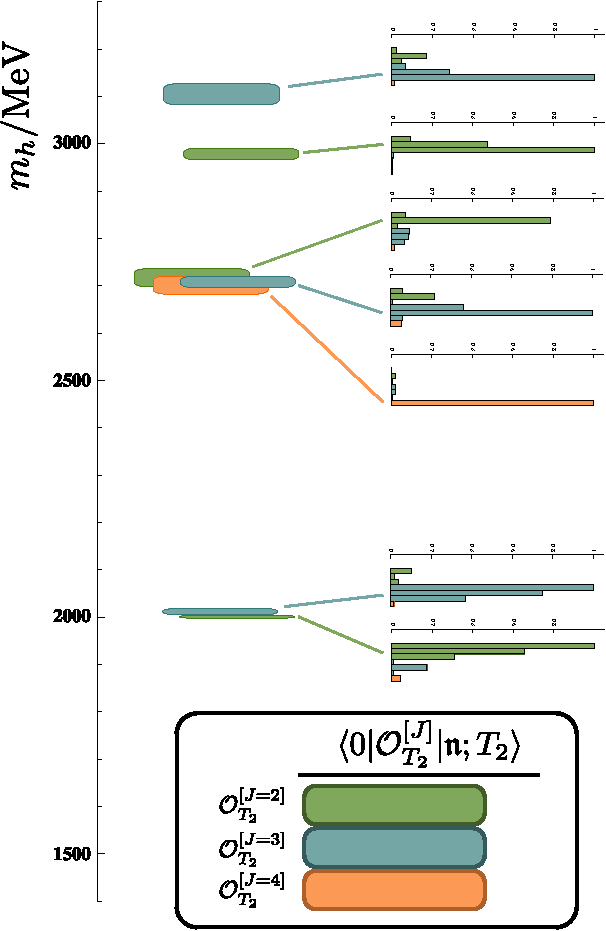
\includegraphics[height=0.6\textheight]{figures/state_ident_T2mP/StateIdent_crop.pdf}
\caption{ State identification in the $\Lambda^{PC} = T_2^{--}$ irrep. Each operator has been normalized, across states, so that $\langle 0 | \mathcal{O}_{T_2} | \estate{n}; T_2 \rangle$ takes a maximal value of one.   \label{fig::StateIdentT2mP}}
\end{centering}
\end{figure}
\clearpage
}

In order to make use of this information we should also show that we do observe the degeneracy previously outlined. This conjectured degeneracy of both masses and operator overlaps is indeed observed in our lattice calculations \cite{Dudek:2010wm,Dudek:2009qf}.  In \figref{fig::J4mMDegen} we show a pattern of  degenerate masses and operator overlaps across the $\Lambda^{PC} = (A_1,T_1,T_2,E)^{-+}$ irreps consistent with a spin-4 meson. We plot the state overlaps with the three derivative operator\footnote{The symbol  $D^{[3]}_{2,3}$ means `construct a three derivative operator, couple the outer two derivatives into $J=2$, then couple the third derivative to make $J=3$'.}
\begin{equation*}
\mathcal{O} \sim  (\epsilon_{ijk} \gamma_i\gamma_j \times D^{[3]}_{2,3})^{J=4} .
\end{equation*}
This is to say an operator in which three gauge covariant derivatives are coupled together to form spin-3 which is then combined with a positive parity vector gamma matrix structure to form $J^{PC} = 4^{-+}$. In all four irreps we find that the tentatively identified $J^{PC}=4^{-+}$ state overlaps predominantly with this operator. Further, we find that the extracted masses and overlaps are statistically compatible across each irrep and indicating the observation of a spin-4 meson. 

\afterpage{
\begin{figure}[htbp]
\begin{centering}
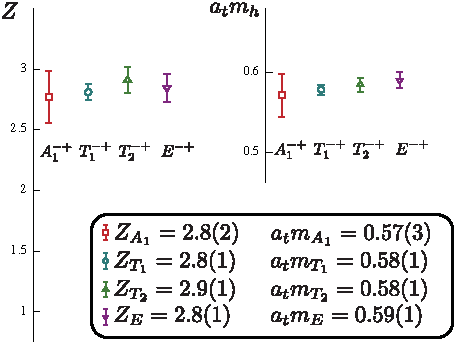
\includegraphics[width=0.8\linewidth]{figures/operator_overlap_degeneracy_J4mM/Degeneracy2.pdf}
\caption{ Degeneracy patterns in the $\Lambda^{PC} = (A_1,T_1,T_2,E)^{-+}$ irreps.\label{fig::J4mMDegen}}
\end{centering}
\end{figure}
\clearpage
}

Turning now to the state identification, the procedure proceeds by identifying the dominant $J$ overlapping with each state. Returning to  \figref{fig::StateIdentT2mP} we explicitly demonstrate the efficacy of our  procedure using a subset of the available operators corresponding to the most relevant constructions. Read, along any single histogram, from top to bottom, the operators are 
% \begin{align*}
%rho_a1xD1_J1__J2_T2 1 0 * \\
%rho_a1xD3_J132_J3__J2_T2 1 0 * \\
%rho_b1xD3_J131_J1__J2_T2 1 0 * \\
%rho_rho_2xD2_J2__J3_T2 1 0 * \\
%rho_a1xD3_J132_J3__J3_T2 1 0 * \\
%rho_b1xD3_J131_J2__J3_T2 1 0 * \\
%rho_a1xD3_J132_J3__J4_T2 1 0 
%\end{align*}
\begin{align*}
\mathcal{O}_{T_2}^{(1),[J=2]} &\sim \left( \gamma_5\gamma_k \times D^{[1]} \right)^{J=2}   \\
\mathcal{O}_{T_2}^{(2),[J=2]} &\sim  \left( \gamma_5\gamma_k \times D^{[3]}_{2,3}\right)^{J=2}   \\
\mathcal{O}_{T_2}^{(3),[J=2]} &\sim  \left( \epsilon_{ijk} \gamma_i\gamma_j \times D^{[3]}_{1,1} \right)^{J=2}   \\
\mathcal{O}_{T_2}^{(4),[J=3]} &\sim  \left( \gamma_0 \gamma_k \times D^{[2]}_2 \right)^{J=3}  \\
\mathcal{O}_{T_2}^{(5),[J=3]} &\sim  \left( \gamma_5\gamma_k \times D^{[3]}_{2,3} \right)^{J=3}   \\
\mathcal{O}_{T_2}^{(6),[J=3]} &\sim  \left( \epsilon_{ijk} \gamma_i\gamma_j \times D^{[3]}_{1,2}\right)^{J=3}   \\
\mathcal{O}_{T_2}^{(7),[J=4]} &\sim  \left( \gamma_5\gamma_k \times D^{[3]}_{2,3}\right)^{J=4} .  
\end{align*}

We find, as might be expected assuming that rotational symmetry is approximately restored, that each state appears to have dominant overlap onto only a single spin. The other irreps, both at rest and in flight, also exhibit similar behavior. By repeating this procedure, identifying the dominant spin component of each state in each irrep, we are able to find the patterns of degenerate states in our lattice calculation. We reproduced the spin identified spectra, for the lowest set of isovector mesons, in Figures \ref{fig::LatticemMSpec743SpinIdent}, \ref{fig::LatticemPSpec743SpinIdent}, \ref{fig::LatticepMSpec743SpinIdent}, and \ref{fig::LatticepPSpec743SpinIdent}. Across each of these plots vertical ellipses represent additional states, present in the spectrum, but whose spin we were unable to unambiguously identify.

%\footnote{The signals for these highly excited states decay rapidly and are often noisy even in the face of the extensive suite of variational tools we have at out disposal.}. 

\afterpage{
\begin{figure}[htbp]
\begin{centering}
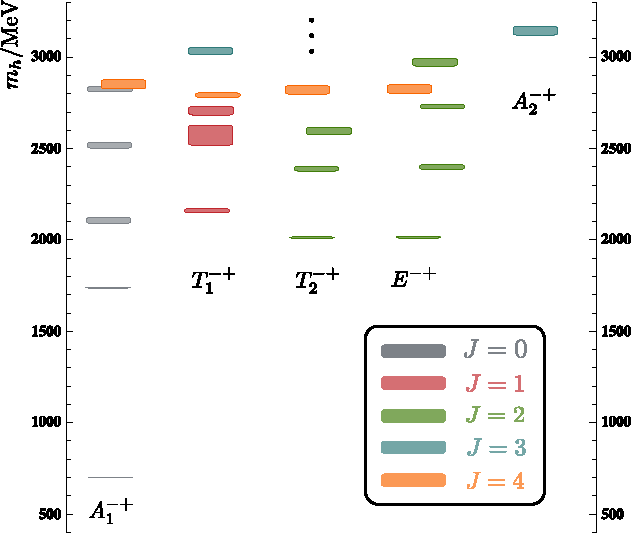
\includegraphics[width=\linewidth]{figures/LatticeSpectrum743/BoxPlotLabeledmM_crop.pdf}
\caption{ Spin identified $J^{PC} = J^{-+}$ $SU(3)_F$ spectrum. \label{fig::LatticemMSpec743SpinIdent}}
\end{centering}
\end{figure}
\clearpage
}

\afterpage{
\begin{figure}[htbp]
\begin{centering}
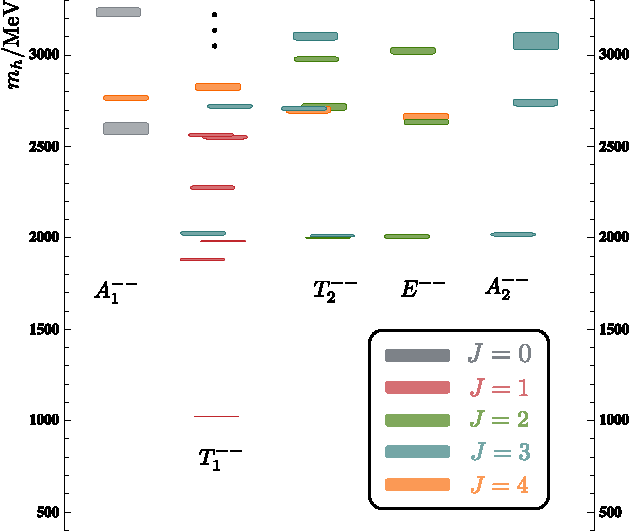
\includegraphics[width=\linewidth]{figures/LatticeSpectrum743/BoxPlotLabeledmP_crop.pdf}
\caption{ Spin identified $J^{PC} = J^{--}$ $SU(3)_F$ spectrum. \label{fig::LatticemPSpec743SpinIdent}}
\end{centering}
\end{figure}
\clearpage
}

\afterpage{
\begin{figure}[htbp]
\begin{centering}
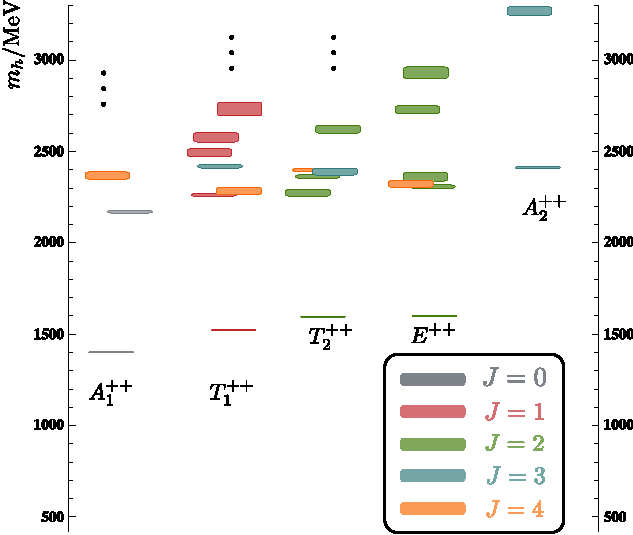
\includegraphics[width=\linewidth]{figures/LatticeSpectrum743/BoxPlotLabeledpM_crop.pdf}
\caption{ Spin identified $J^{PC} = J^{++}$ $SU(3)_F$ spectrum. \label{fig::LatticepMSpec743SpinIdent}}
\end{centering}
\end{figure}
\clearpage
}

\afterpage{
\begin{figure}[htbp]
\begin{centering}
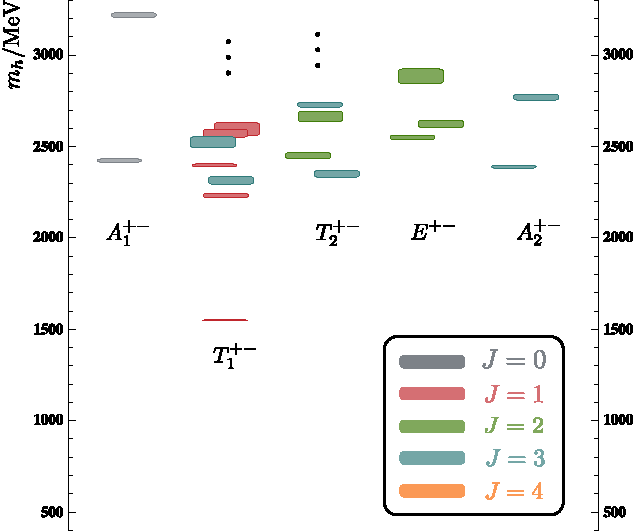
\includegraphics[width=\linewidth]{figures/LatticeSpectrum743/BoxPlotLabeledpP_crop.pdf}
\caption{ Spin identified $J^{PC} = J^{+-}$ $SU(3)_F$ spectrum. \label{fig::LatticepPSpec743SpinIdent}}
\end{centering}
\end{figure}
\clearpage
}
%%%%%%%%%%%%%%%%%%%%%%%%%%%%%%%%%%%%%%%%%%%%%%%%%%%%%%%%%
%%%%%%%%%%%%%%%%%%%%%%%%%%%%%%%%%%%%%%%%%%%%%%%%%%%%%%%%%
%%%%%%%%%%%%%%%%%%%%%%%%%%%%%%%%%%%%%%%%%%%%%%%%%%%%%%%%%

\section{$SU(3)_F$ Spectrum} \label{sec::Spec:results}

We conclude this chapter by presenting the spin identified $SU(3)_F$ spectrum.  

\afterpage{
\begin{figure}[htbp]
\begin{centering}
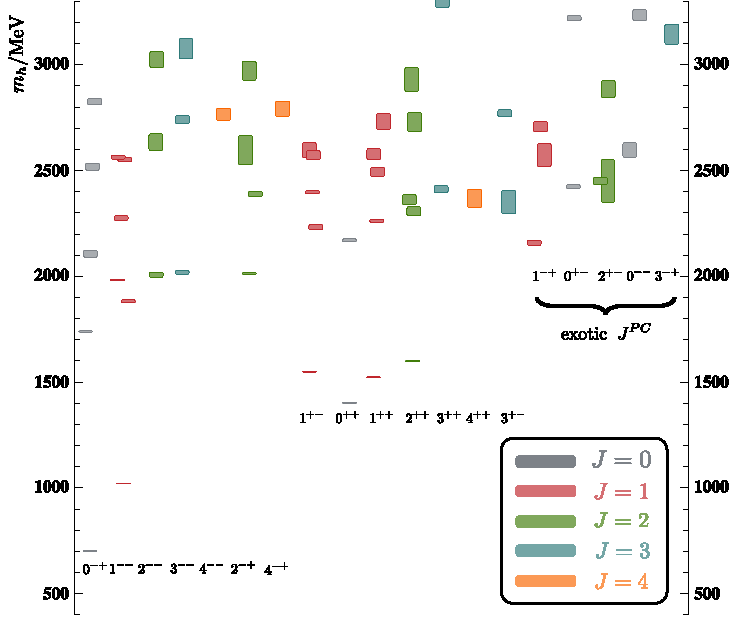
\includegraphics[width=\linewidth]{figures/LatticeSpectrum743/SpinIdentAll.pdf}
\caption{ Spin identified $J^{PC}$ $SU(3)_F$ spectrum. \label{fig::LatticeSpec743SpinIdent}}
\end{centering}
\end{figure}
\clearpage
}

